\documentclass[a4paper]{article}
\usepackage{amsmath}
\usepackage{amssymb}
\usepackage{amsthm}
\usepackage{amsfonts}
\usepackage[margin=1in]{geometry}
\usepackage{graphicx}
\usepackage{algorithm}
\usepackage[noend]{algpseudocode}
\allowdisplaybreaks
\usepackage{babel}
\usepackage{bbm}
\usepackage{float}
\usepackage{subfig}

\allowdisplaybreaks
\graphicspath{ {./imgs/} }


\begin{document}

\title{Intro to Signal Processing -- HW4}
\author{Yinon Goldshtein , Roee Idan}
\date{Submitted to January 26 2023}
\maketitle

\part{Theory}

\section*{Question 1 -- Inverting the Second Derivative Operator}



\subsection*{a}
\begin{align}
        H = \begin{pmatrix} \frac{-5}{2} & \frac{4}{3} & \frac{-1}{12} & 0 &\cdots & 0 & \frac{-1}{12} & \frac{4}{3}\\ \frac{4}{3} & \frac{-5}{2} & \frac{4}{3} & \frac{-1}{12}& 0 & \cdots & 0 & \frac{-1}{12} \\ \frac{-1}{12} & \frac{4}{3} & \frac{-5}{2} & \frac{4}{3} & \ddots & 0 & \cdots & 0 \\ 0 & \frac{-1}{12} & \frac{4}{3} & \frac{-5}{2} & \frac{4}{3} & \cdots & 0 & \vdots \\ \vdots & \ddots & \ddots & \ddots &\ddots & \ddots & \ddots & \vdots \\ \frac{4}{3} & \frac{-1}{12} & 0 & \cdots & 0 & \frac{-1}{12} & \frac{4}{3} & \frac{-5}{2}
    \end{pmatrix}
\end{align}



\subsection*{b}
Because H is a circulant we get that it is diagnalizable with the DFT matrix and so $H = DFT \times \Lambda \times DFT^{*}$. We know that the first row of $H_{0}$ is
\begin{align}
    H_{0} = \begin{pmatrix} \frac{-5}{2} \\ \frac{4}{3} \\ \frac{-1}{12} \\ 0 \\ \vdots \\0 \\ \frac{-1}{12} \\ \frac{4}{3}
    \end{pmatrix}
\end{align}
From here we can deduce that
\begin{align}
    \Lambda = \sqrt{M} \times DFT^{*} \times H_{0} = \begin{pmatrix}
        \sum_{l=0}^{M-1}W_{M}^{0,l}H_{0} \\ \sum_{l=0}^{M-1}W_{M}^{1,l}H_{0} \\ \vdots \\
        \sum_{l=0}^{M-1}W_{M}^{M-1,l}H_{0}
    \end{pmatrix} = \begin{pmatrix}
        0 \\ \sum_{l=0}^{M-1}W_{M}^{1,l}H_{0} \\ \vdots \\
        \sum_{l=0}^{M-1}W_{M}^{M-1,l}H_{0}
    \end{pmatrix}
\end{align}

We know that the rank of $H$ is $M-1$ and so we can deduce that $\Lambda_{0}$ is the only zero and beacause we know that $H$ is symmetric we can deduce that all the eigenvalues  are real and so the Psuedo inverse of H will be 
\begin{align}
    H^{+} = DFT \times \Lambda^{+} \times DFT^{*}
\end{align}
where we define $\Lambda^{+}$ to be 0 in all places that aren't the diagonal and in the diagonal:
\begin{align}
    diag(\Lambda^{+}) = \begin{pmatrix}
        0 \\ \frac{1}{\sum_{l=0}^{M-1}W_{M}^{1,l}H_{0}} \\ \vdots \\
        \frac{1}{\sum_{l=0}^{M-1}W_{M}^{M-1,l}H_{0}} \end{pmatrix}
\end{align}



\subsection*{c}
Using the previously provided inverse filter $\varphi$ cannot be perfectly recovered due to the fact that $H$ has a null space which from what we learnt is not invertible and from here we can deduce that any signal that part of its component will be in the null space cannot be recovered. So for example we can build a signal which is a scaled version of the eigenvector that is corresponding to the eigenvalue of 0 and which will be the first row of $DFT^{*}$ and so for $c \neq 0$ we get that
\begin{align}
    \varphi := c \begin{pmatrix}
        W^{0}_{M} \\ W^{0}_{M} \\ \vdots \\ W^{0}_{M}
    \end{pmatrix} = \begin{pmatrix}
        c \\ c \\ \vdots \\ c
    \end{pmatrix}
\end{align}

We can see that for this $\varphi$ we get that $H \times \varphi = 0$ and also for all $c \neq 0$ we will get that
\begin{align}
    \varphi \neq H^{+} \times H \times \varphi = 0
\end{align}


\newpage
\section*{Question 2 -- Let’s Randomise}


\subsection*{a}
Let us look at the expected value for each value and let us show that they are all $0$.
Let us look first $i \leq \frac{N}{2}$ we get that :
\begin{align}
    E[\varphi_{i}] &= E[\varphi_{i} | K=i] P(K=i) + E[\varphi_{i} | K\neq i] P(K \neq i) =
    E[M+L_{1}] P(K=i) + E[M] P(K \neq i) = \nonumber \\[2ex] 
    &= (E[M]+E[L_{1}]) P(K=i) + E[M] P(K \neq i) = 0
\end{align}

Let us look first $i > \frac{N}{2}$ we get that :
\begin{align}
    E[\varphi_{i}] &= E[\varphi_{i} | K=i] P(K=i) + E[\varphi_{i} | K\neq i] P(K \neq i) =
    E[M+L_{2}] P(K=i) + E[M] P(K \neq i) = \nonumber \\[2ex] 
    &= (E[M]+E[L_{2}]) P(K=i) + E[M] P(K \neq i) = 0
\end{align}
And from here can deduce that random vector $\varphi$ has a zero mean



\subsection*{b}
From the question's information we get that $R_{\varphi}$ matrix will $R_{\varphi}=E[\varphi \varphi^{T}]$ let us denote in $R_{\varphi}$ $r_{i.j}$ as the element in the place $i,j$. Let us note that $M, L$ are independent and also that $E[M]=E[L]=0$. When $i \neq j$ we get that:
\begin{align}
    r_{i,j} &= E[\varphi_{i}\varphi_{j}] = E[\varphi_{i}\varphi_{j}|K=i]P(K=i) + E[\varphi_{i}\varphi_{j}|K=j]P(K=j) + E[\varphi_{i}\varphi_{j}|K \neq i,j]P(K\neq i,j) = \nonumber \\[2ex] &= E[(M+L)M]P(K=i) + E[M(M+L)]P(K=j) + E[M^{2}]P(K\neq i,j) = \nonumber \\[2ex] &=  (E[M^{2}]+E[L]E[M])P(K=i) + (E[M^{2}]+E[M]E[L])P(K=j) + E[M^{2}]P(K\neq i,j) = \nonumber \\[2ex] &= E[M^{2}]P(K=i) + P(K=j) + P(K\neq i,j) = E[M^{2}] = c
\end{align}
When $i = j$ we get that:
\begin{align}
    r_{i,j} &= E[\varphi_{i}\varphi_{i}|K=i]P(K=i) + E[\varphi_{i}\varphi_{i}|K \neq i]P(K \neq i) = 
    E[(M+L)(M+L)]P(K=i) + E[M^{2}]P(K \neq i) = \nonumber \\[2ex] &= (E[M^{2}]+2E[M]E[L]+E[L^{2}])P(K=i) + E[M^{2}]P(K \neq i)
\end{align}
And from here we get that when $i \leq \frac{N}{2}$
\begin{align}
    r_{i,j} = E[M^{2}]+\frac{E[L_{1}^{2}]}{N} = a + c
\end{align}
and when $i > \frac{N}{2}$ 
\begin{align}
    r_{i,j} = E[M^{2}]+\frac{E[L_{2}^{2}]}{N} = b + c
\end{align}



\subsection*{c}
In order for the $PCA$ to be $DFT^{*}$ we need that $R_{\varphi}$ should be diagonalizable with $DFT^{*}$ which will occur if and only if $R_{\varphi}$ is circulant and so for that to happened we will need that $a = b$ 



\newpage
\section*{Question 3 -- Let’s Randomise Again!}

Now the signal $\varphi$ is: 

\begin{align*}
    \varphi = \begin{bmatrix} M & \cdots & M+L & M & \cdots & M & M+L & M & \cdots & M \end{bmatrix}^T
\end{align*}

Where the $M+L$ terms appear in the $K$-th and the $(K+\frac{N}{2})$-th elements.

\subsection*{a}

Available random variables: $K \sim U(\{1,\dots,\frac{N}{2}\}), \mathbb{E}(M)=0, \mathbb{E}(M^2)=c, \mathbb{E}(L)=0, \mathbb{E}(L^2)=\frac{N}{2}(1-c)$. \\
$c$ is a real constant $c\in(0,1)$.

We know that $K,M,L$ are independent, therefore:

\begin{align*}
    & \mathbb{E}(L\cdot M)=\mathbb{E}(L)\cdot \mathbb{E}(M)=0 \\
    & \mathbb{E}(M(M+L))=\mathbb{E}(M^2)+\mathbb{E}(LM)=\mathbb{E}(M^2)=c \\
    & \mathbb{E}((M+L)^2)=\mathbb{E}(M^2+2LM+L^2)=\mathbb{E}(M^2)+\mathbb{E}(2LM)+\mathbb{E}(L^2) = c+\frac{N}{2}(1-c)
\end{align*}

Now we can calculate the autocorrelation matrix by: $R_\varphi = \mathbb{E}(\varphi \varphi^T)$

\begin{align*}
    \varphi \varphi^T = 
    \begin{pmatrix}
        M^2 & \cdots & M^2 & M(M+L) & M^2 & \cdots & M^2 & M(M+L) & M^2 & \cdots  M^2 \\ 
        \vdots & \vdots & \vdots & \vdots & \vdots & \vdots & \vdots & \vdots & \vdots & \vdots \\
        M(M+L) & \cdots & \cdots & (M+L)^2 & \cdots & \cdots & M(M+L) & (M+L)^2 & \cdots & M(M+L) \\
        M^2 & \cdots  & & & & & & & \cdots & M^2
    \end{pmatrix}
\end{align*}


So actually, the $K$ and $K+\frac{N}{2}$ columns and rows are:

\begin{align*}
    [\varphi \varphi^T]_{i,j}=
    \begin{cases}
        (M+L)^2 ,\quad i\in \{K, K+\frac{N}{2}\}, j\in \{K, K+\frac{N}{2}\} \\
        M(M+L) , \quad i,j\in \{K, K+\frac{N}{2}\} \\
        M^2 , \quad otherwise
    \end{cases}
\end{align*}

And so the auto-correlation matrix, which is $R_\varphi = E[\varphi \varphi^T]$ is:

\begin{align*}
    & [R_\varphi]_{i,j}= \mathbb{E}(\varphi_i \cdot \varphi_j) \\
    & (1)\quad i=j \implies R_{i,j} = \mathbb{E}(\varphi_i^2) = \\
    & \mathbb{E}(\varphi_i^2 \mid i\neq {K,K+\frac{N}{2}}) \cdot P(i\neq {K,K+\frac{N}{2}}) + \mathbb{E}(\varphi_i^2 \mid i= {K,K+\frac{N}{2}}) \cdot P(i= {K,K+\frac{N}{2}}) = \\
    & E(M^2) \cdot \frac{N-2}{N} + E((M+L)^2) \cdot \frac{2}{N} = 
    c \cdot \frac{N-2}{N} + \frac{2}{N} \cdot (c+\frac{N}{2}\cdot(1-c)) = \\
    & c+1-c = 1 \\
    & (2)\quad i-j=\frac{N}{2}\mod N (\text{The N/2 diagonal}) \implies R_{i,j}=\mathbb{E}(\varphi_i \varphi_j) = \\ 
    & \mathbb{E}(\varphi_i \varphi_j \mid i,j\neq {K,K+\frac{N}{2}}) \cdot P(i,j\neq {K,K+\frac{N}{2}}) + \mathbb{E}(\varphi_i \varphi_j \mid i,j = {K,K+\frac{N}{2}}) \cdot P(i,j = {K,K+\frac{N}{2}}) \underbrace{=}_{*} \\
    & \mathbb{E}(M^2) \cdot \frac{N-2}{N} + \mathbb{E}((M+L)^2)\cdot \frac{2}{N} =
    c \cdot \frac{N-2}{N} + \frac{2}{N} \cdot (c+\frac{N}{2}\cdot (1-c)) = 1 \\
    & (3) \quad i-j\neq\frac{N}{2}\mod N \land i\neq j (\text{otherwise}) \implies R_{i,j} = \mathbb{E}(\varphi_i \varphi_j) = \\
    & \mathbb{E}(\varphi_i \varphi_j \mid i=K,K+\frac{N}{2})\cdot P(i=K,K+\frac{N}{2}) + \mathbb{E}(\varphi_i \varphi_j \mid j=K,K+\frac{N}{2})\cdot P(j=K,K+\frac{N}{2}) + \\ & \mathbb{E}(\varphi_i \varphi_j \mid i,j\neqK,K+\frac{N}{2})\cdot P(i,j\neq K,K+\frac{N}{2}) = \\
    & \mathbb{E}(M(L+M))\cdot \frac{2}{N} \cdot 2 + \frac{N-4}{N} \cdot \mathbb{E}(M^2) = c \cdot \frac{4}{N} + c\cdot \frac{N-4}{N} = c
\end{align*}

So in conclusion:

\begin{align*}
    & [R_\varphi]_{i,j}=
    \begin{cases}
        1 ,\quad \text{Main diagonal, or $\pm\frac{N}{2}$ diagonals } \\
        c , \quad otherwise
    \end{cases} \\
    & \text{Row 0 of $R_\varphi$ is:} \\
    & \begin{pmatrix}
        1 & c & \cdots & c & 1 & c & \cdots & c
    \end{pmatrix}
\end{align*}

And every following row is the previous row, shifted right by one element (in row 2 the 1 is in the second position).

Therefore, $R_\varphi$ is circulant with a period of $\frac{N}{2}$.


\subsection*{b}

We saw in HW3 that the eigenvalues of $R_\varphi$, stacked in a column, equals to the product of the $DFT^*$ matrix and the first row of $R_\varphi$ rewritten in column form, normalized by the root of the size of $R_\varphi$. Therefore: \\

\begin{align*}
    \begin{pmatrix}
        \lambda_0 \\ \vdots \\ \lambda_{N-1}
    \end{pmatrix} = 
    \sqrt(N) \cdot DFT^* \cdot \begin{pmatrix}
        1 & c & \cdots & c & 1 & c & \cdots & c
    \end{pmatrix} ^T
\end{align*}

\newpage
\section*{Question 4 -- Wiener Filter}


\subsection*{a}
We know that $\varphi^{*} = H \varphi + n$ and so the autocorrelation will be defined by:
\begin{align}
    R_{\varphi^{*}} &= E(\varphi \varphi^{*}) = E(( H \varphi + n)( H \varphi + n)^*) = E(( H \varphi + n)( H^{*} \varphi^{*} + n^{*})) = \nonumber \\[2ex] 
    &= E(H\varphi\varphi^{*}H^{*}+H\varphi n^{*} + n \varphi^{*}H^{*}+ nn^{*}) = \nonumber \\[2ex] 
    &= E(H\varphi\varphi^{*}H^{*})+E(H\varphi n^{*}) + E(n \varphi^{*}H^{*}) + E(nn^{*}) = \nonumber \\[2ex] 
    &= H E(\varphi)E(\varphi^{*})H^{*}+H E(\varphi)E( n^{*}) + E(n) E(\varphi^{*})H^{*} + E(nn^{*})  = \nonumber \\[2ex] 
    &= H R_{\varphi} H^{*} + R_{n}
\end{align}
\subsection*{b}
For the case $R_{n} = \sigma_{n}^{2}$I is from what we learned in class to be and from  what we saw in the previous subsection we get that
\begin{align}
    W = R_{\varphi}H^{*}(HR_{\varphi}H^{*}+\sigma^{2}_{n}I)^{-1} =  = R_{\varphi} H^{*} R^{-1}_{\varphi^{*}}
\end{align}
\subsection*{c}
We get that for $A = DFT \Lambda DFT^{*}$ because by definition $W^{l}_{N}=W^{l (mod N)}_{N}$
\begin{align}
    a_{i,j} = \sum_{k=0}^{N-1}W_{N}^{-ik}\lambda_{k}W_{N}^{-jk} = \sum_{k=0}^{N-1}\lambda_{k}W_{N}^{k(j-i)} =  \sum_{k=0}^{N-1}\lambda_{k}W_{N}^{k(j-i)(mod N)} = a_{0,(j-i)(mod N)}
\end{align}

and from here we can deduce that A will be a circulant matrix.
\subsection*{d}
The Wiener  filter is not a shift invariant system, for example for the case that
$R_{\varphi} = \begin{pmatrix}
        1 & 0 \\ 
        0 & 1
    \end{pmatrix}$, $H_{\varphi} = \begin{pmatrix}
        0 & 1 \\ 
        0 & 0
    \end{pmatrix}$ and $\sigma^2_n = 1$ we will get from calculation that the filter will be from the equation

\begin{align}
    W &= R_{\varphi}H^{*}(HR_{\varphi}H^{*}+\sigma^{2}_{n}I)^{-1} = \begin{pmatrix}
        1 & 0 \\ 
        0 & 1
    \end{pmatrix}\begin{pmatrix}
        0 & 0 \\ 
        1 & 0
    \end{pmatrix}(\begin{pmatrix}
        0 & 1 \\ 
        0 & 0
    \end{pmatrix}\begin{pmatrix}
        1 & 0 \\ 
        0 & 1
    \end{pmatrix}\begin{pmatrix}
        0 & 0 \\ 
        1 & 0
    \end{pmatrix}+\begin{pmatrix}
        1 & 0 \\ 
        0 & 1
    \end{pmatrix})^{-1} = \begin{pmatrix}
        0 & 0 \\ 
        0.5 & 0
    \end{pmatrix}
\end{align}

Note that the Wiener filter is not circulant and so from what we learned we can deduce that it is not a shift invariant.
\subsection*{e}
Let us note $A,B$ as circulant matrixes. we get that also $A^{*},B^{*}$ are also circulant and we get as well that
\begin{align}
    A^{-1} = ((DFT) \Lambda (DFT^{*}))^{-1} = (DFT) \Lambda^{-1} (DFT^{*})    
\end{align}
and so we get that $A^{-1},B^{-1}$ are also circunt also we can calculate that
\begin{align}
    A  + B = (DFT) \Lambda_{A} (DFT^{*}) + (DFT) \Lambda_{B} (DFT^{*}) = (DFT) (\Lambda_{A} + \Lambda_{B}) (DFT^{*})
\end{align}
and so we get that $A+B$ is also circulant also we can calculate that
\begin{align}
    AB = (DFT) \Lambda_{A} (DFT^{*}) \times (DFT) \Lambda_{B} (DFT^{*}) = (DFT) (\Lambda_{A}\Lambda_{B}) (DFT^{*})
\end{align}
and so we get that $AB$ is also circulant. also not that for every $\sigma_{n}^{2}$ we get that $\sigma_{n}^{2}I$ is circulant.
From here we can deduce that the condition will be that $R_{\varphi}$ and $H$ will be circulant inorder for the Wiener filter to be shift-invariant. 
\newpage
\part{Implementation}

\section*{a}

Given the possible sample sizes of $[200, 500, 2000, 5000]$, the mean signal and autocorrelation matrices are:

\begin{figure}[h]
    \centering
    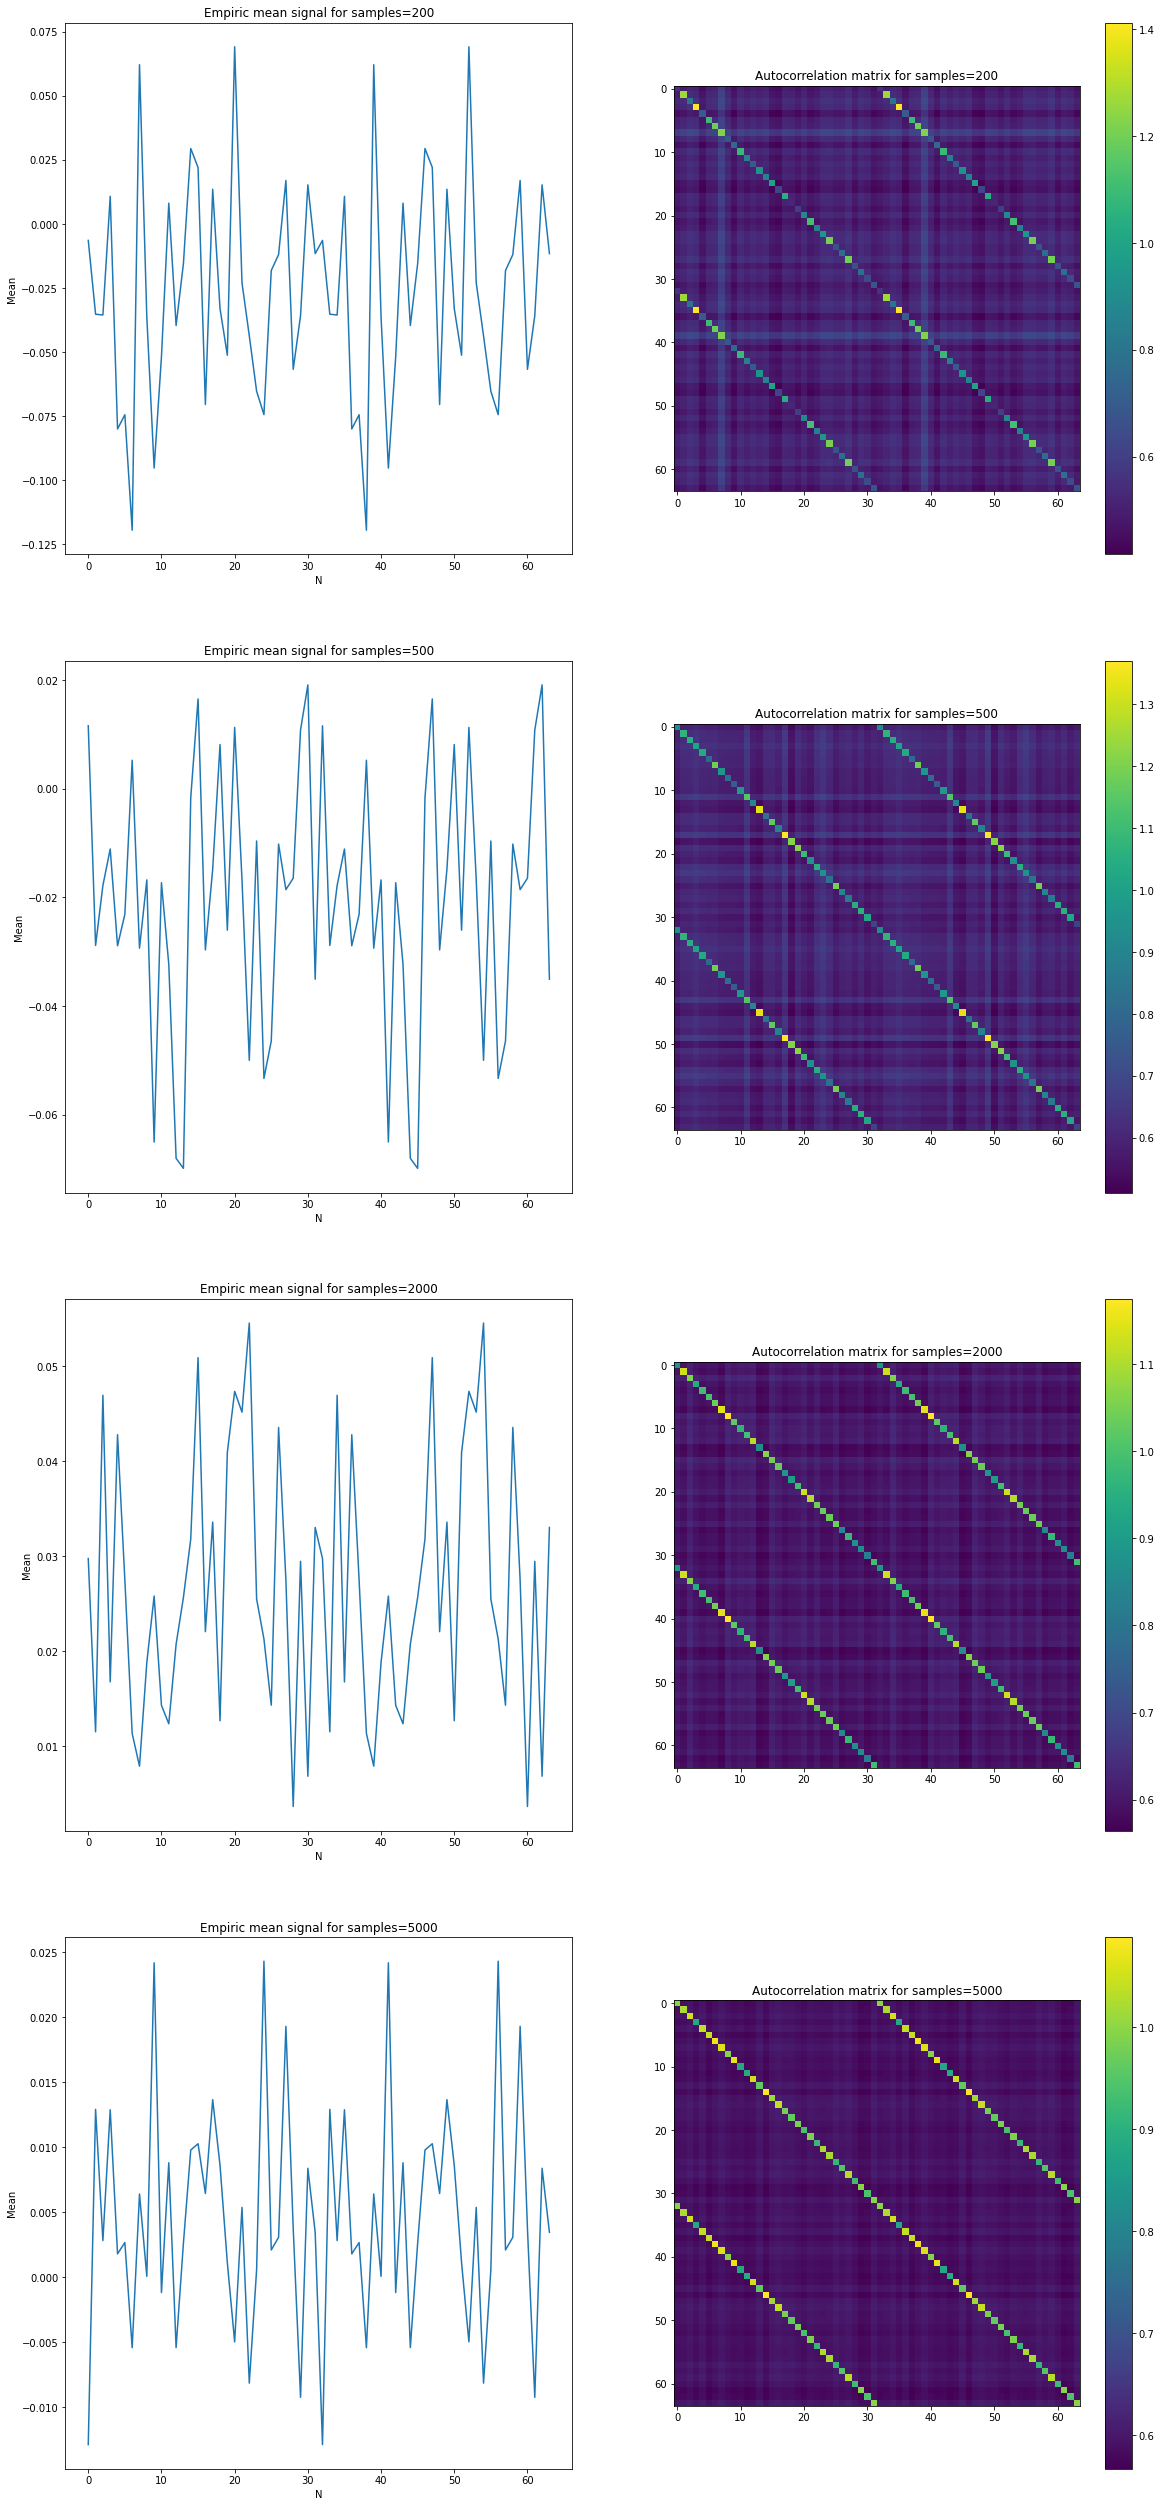
\includegraphics[width=0.78\textwidth,height=0.78\textheight,keepaspectratio]{p2q1a.png}
\end{figure}

As expected, we can see that our theory holds more when the sample size increases. \\
Looking at our max sample size which is $num=5000$, we can see in the auto-correlation matrix that almost all values not on the three "special" diagonals are approximately $\approx c=0.6$, and the values on the diagonals are approximately $\approx 1$. 

In our mean signal figure, we can see that the mean is $0\pm 0.025$, which is centered quite good.

From here, we proceed with our values using sample size=5000.


\section*{b}

The Wiener filter matrix that we obtained:

\begin{figure}[h]
    \centering
    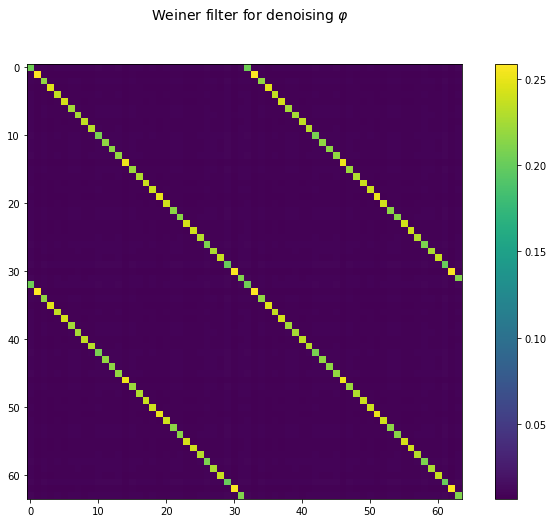
\includegraphics[width=350,keepaspectratio]{p2q1b_weiner.png}
\end{figure}

In this section, our linear degradation matrix is $H=I$, so the Weiner filter's formal calculation will be: $W=R_\varphi \cdot \big( R_\varphi + \sigma_n^2 \cdot I \big) ^ {-1}$

We can also see that the Weiner matrix is circulant, in according to Q4 in the dry part - where if the auto-correlation is circulant, the weiner matrix is circulant.

\newpage 

This is a plot of 10 random signal samples, with their corresponding noisy and denoised signals:

\begin{figure}[h]
    \centering
    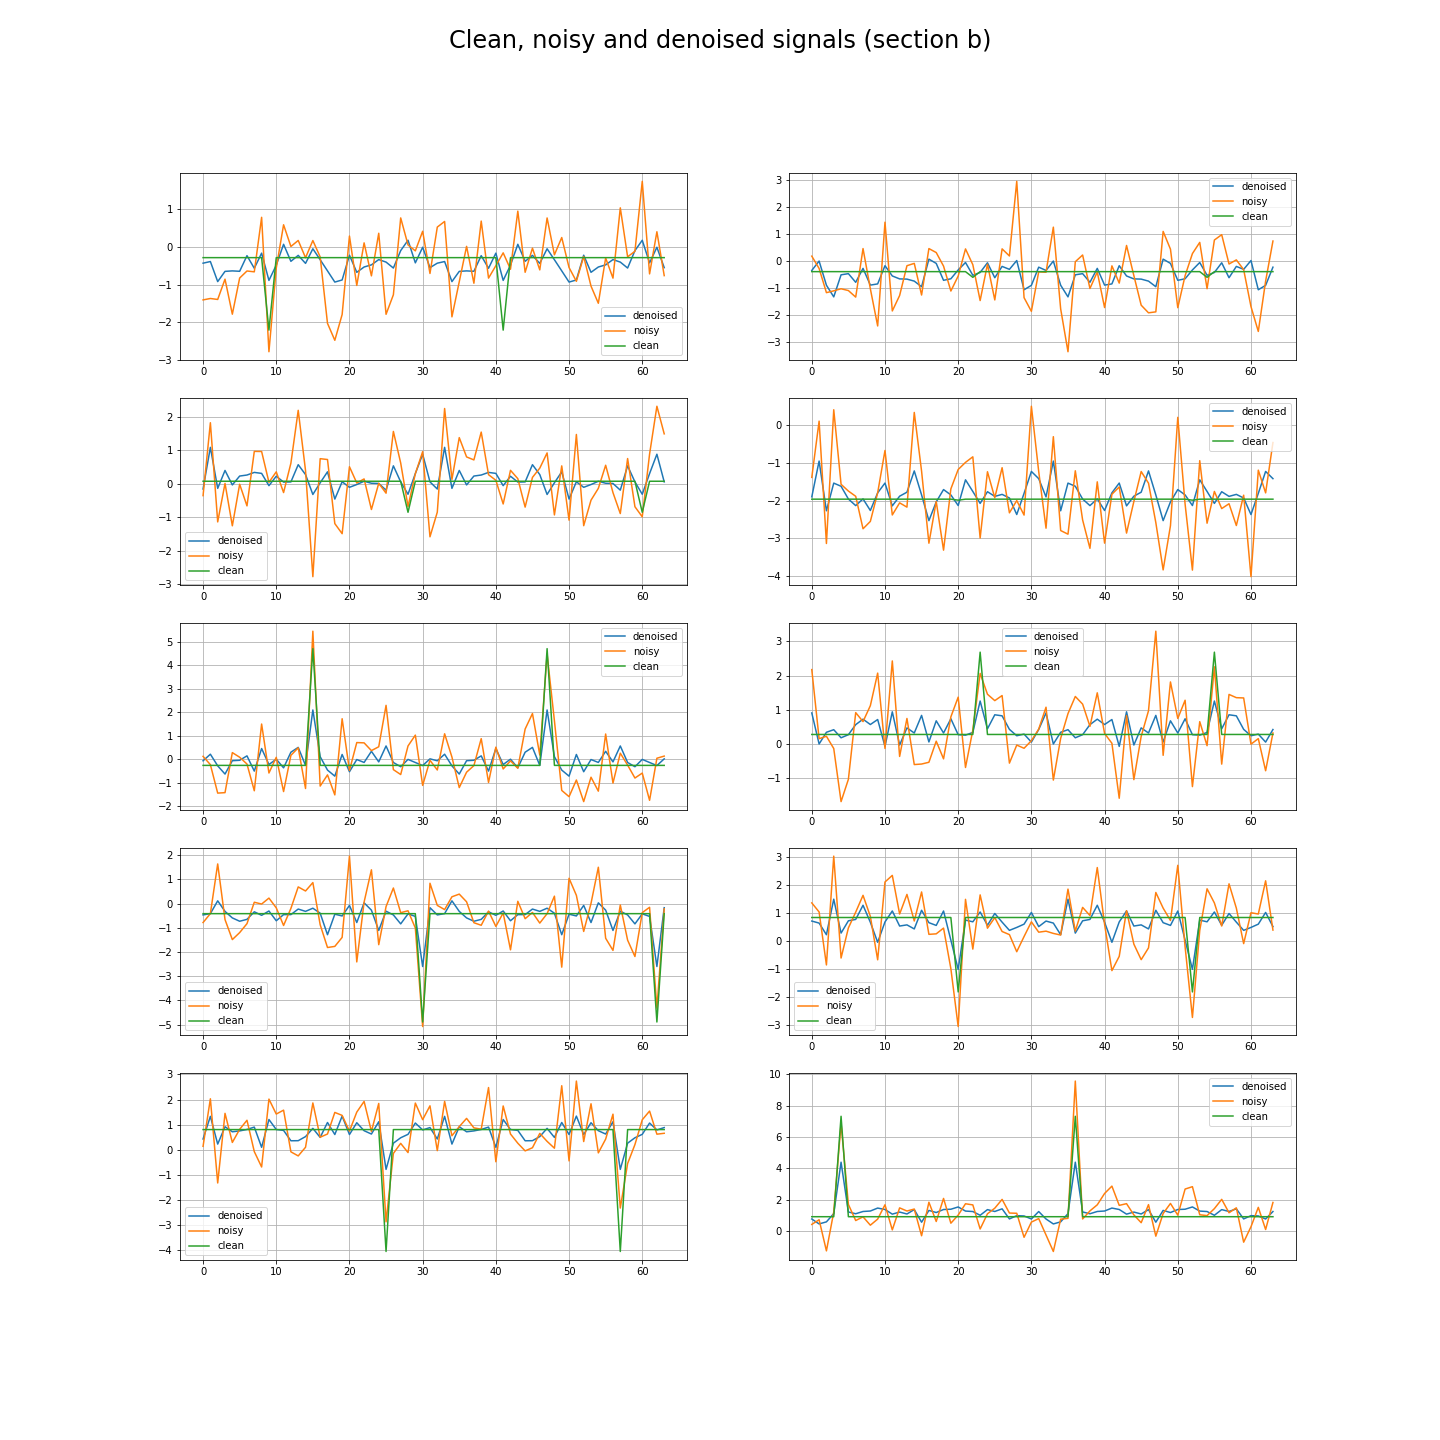
\includegraphics[width=500,keepaspectratio]{samples_b.png}
\end{figure}

The mean MSE of all Weiner-denoised signals with respect to the original signals is: 0.229

This result is good, as the MSE is an order of magnitude lower than the variance of the noise.

\newpage

\section*{c}

The Wiener filter matrix that we obtained:

\begin{figure}[h]
    \centering
    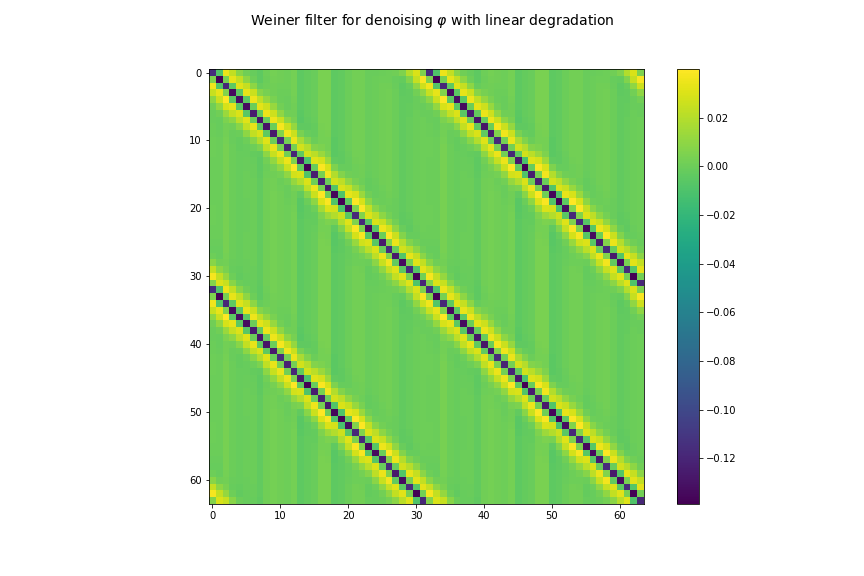
\includegraphics[width=350,keepaspectratio]{p2q1c_weiner.png}
\end{figure}

In this section, our linear degradation matrix is a circulant matrix with a first row of \\ \begin{bmatrix}
    -\frac{5}{2} & \frac{4}{3} & -\frac{1}{12} & 0 & \dots & 0 & -\frac{1}{12} & \frac{4}{3}
\end{bmatrix}, so the Weiner filter's formal calculation will be: \\
$W=R_\varphi \cdot H^T \cdot \big(H\cdot R_\varphi \cdot H^T + \sigma_n^2 \cdot I \big) ^ {-1}$

We can also see that the Weiner matrix is circulant, in according to Q4 in the dry part - where if the auto-correlation is circulant, the weiner matrix is circulant.


\newpage 

This is a plot of 10 random signal samples, with their corresponding noisy and denoised signals:

\begin{figure}[h]
    \centering
    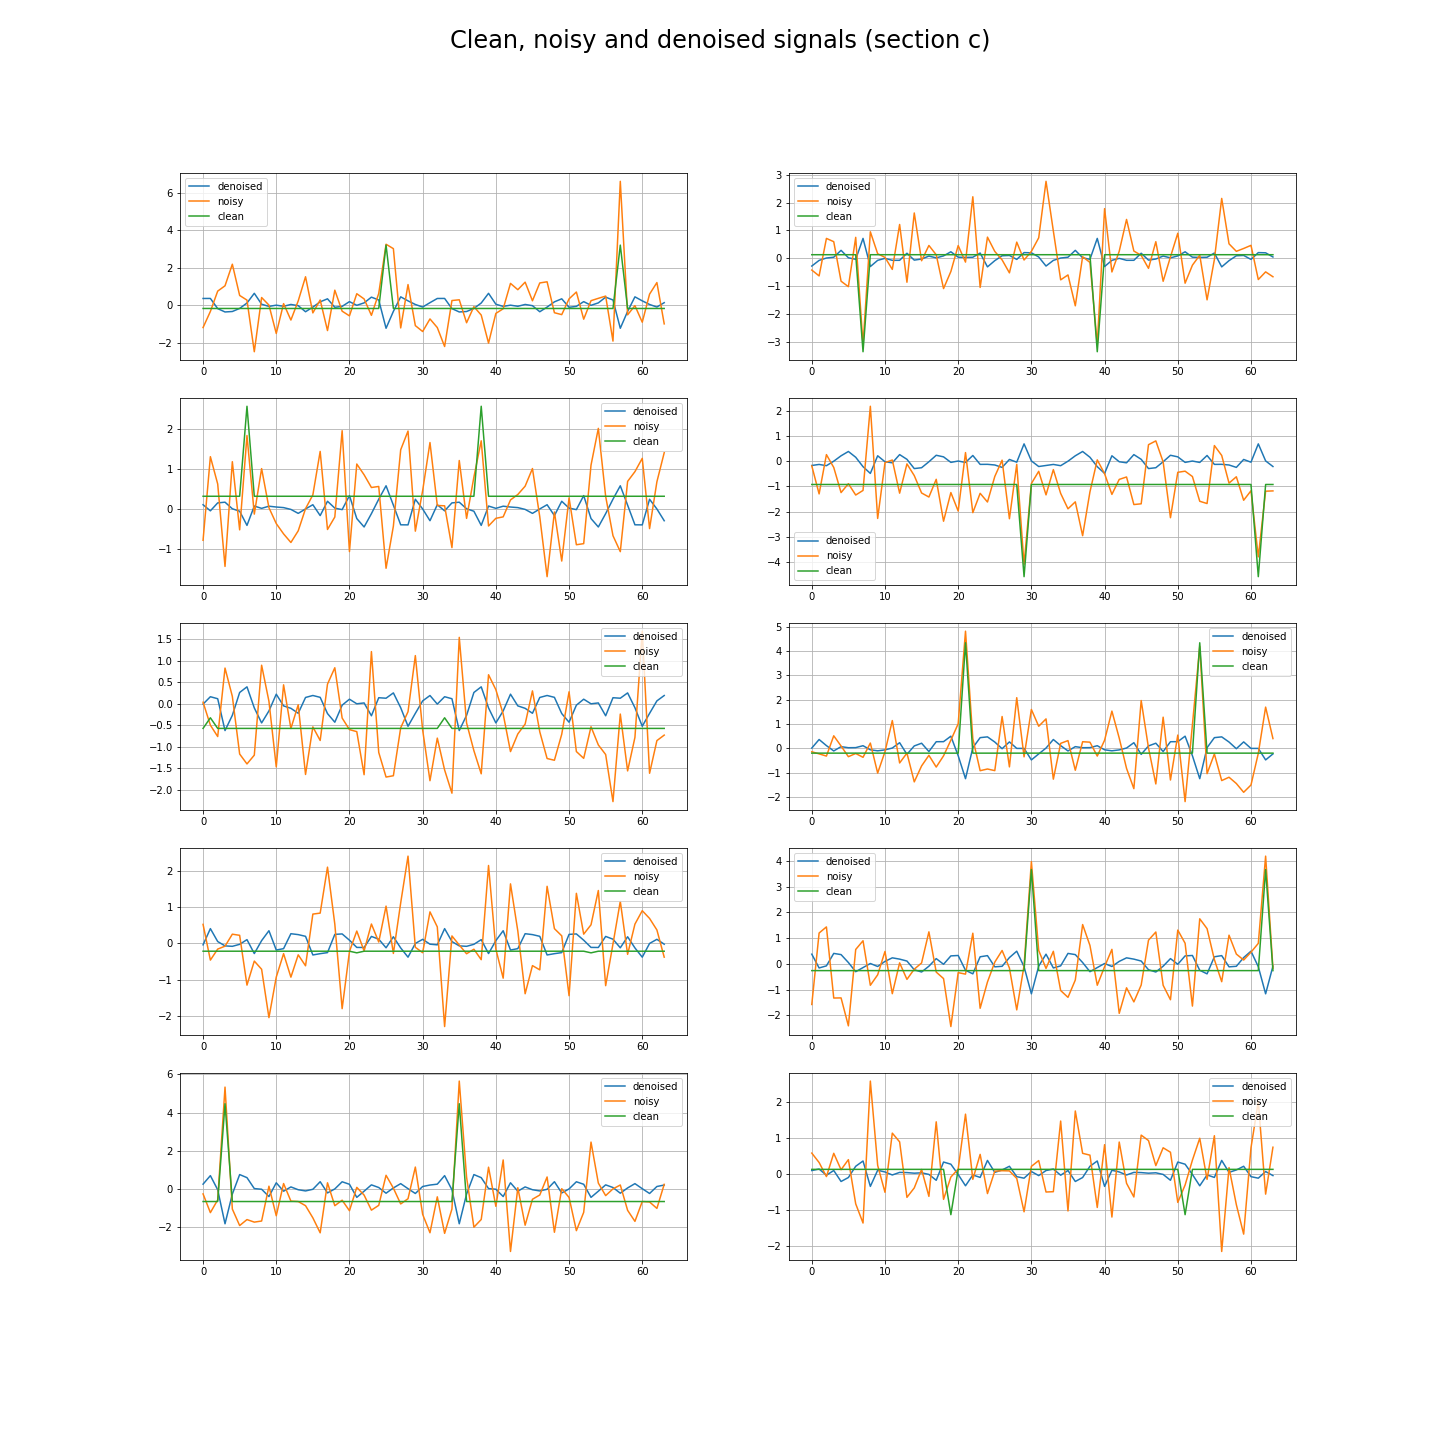
\includegraphics[width=500,keepaspectratio]{samples_c.png}
\end{figure}

The mean MSE of all Weiner-denoised signals with respect to the original signals is: 1.275

This result is worse then before, when we calculated the MSE without the added linear degradation. This is because H is not invertible, because now the parts of the vectors that corresponds to the eigenvector of the eigenvalue 0 are degraded and lost.


\newpage 

\section*{d}

\subsection*{Without linear degradation}

The Wiener filter matrix that we obtained:

\begin{figure}[h]
    \centering
    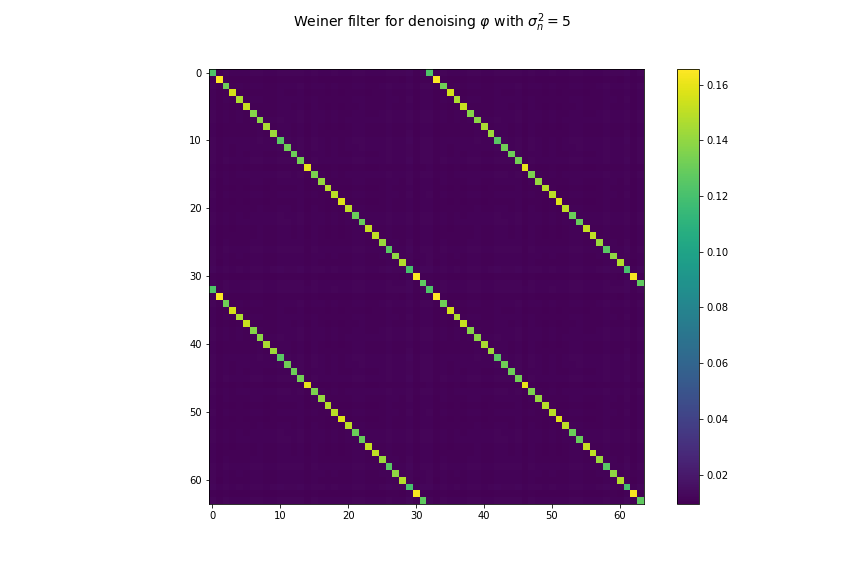
\includegraphics[width=350,keepaspectratio]{p2q1d_weiner_one.png}
\end{figure}

In this section, our linear degradation matrix is $H=I$, so the Weiner filter's formal calculation will be: $W=R_\varphi \cdot \big( R_\varphi + \sigma_n^2 \cdot I \big) ^ {-1}$

We can also see that the Weiner matrix is circulant, in according to Q4 in the dry part - where if the auto-correlation is circulant, the weiner matrix is circulant.


\newpage 

This is a plot of 10 random signal samples, with their corresponding noisy and denoised signals:

\begin{figure}[h]
    \centering
    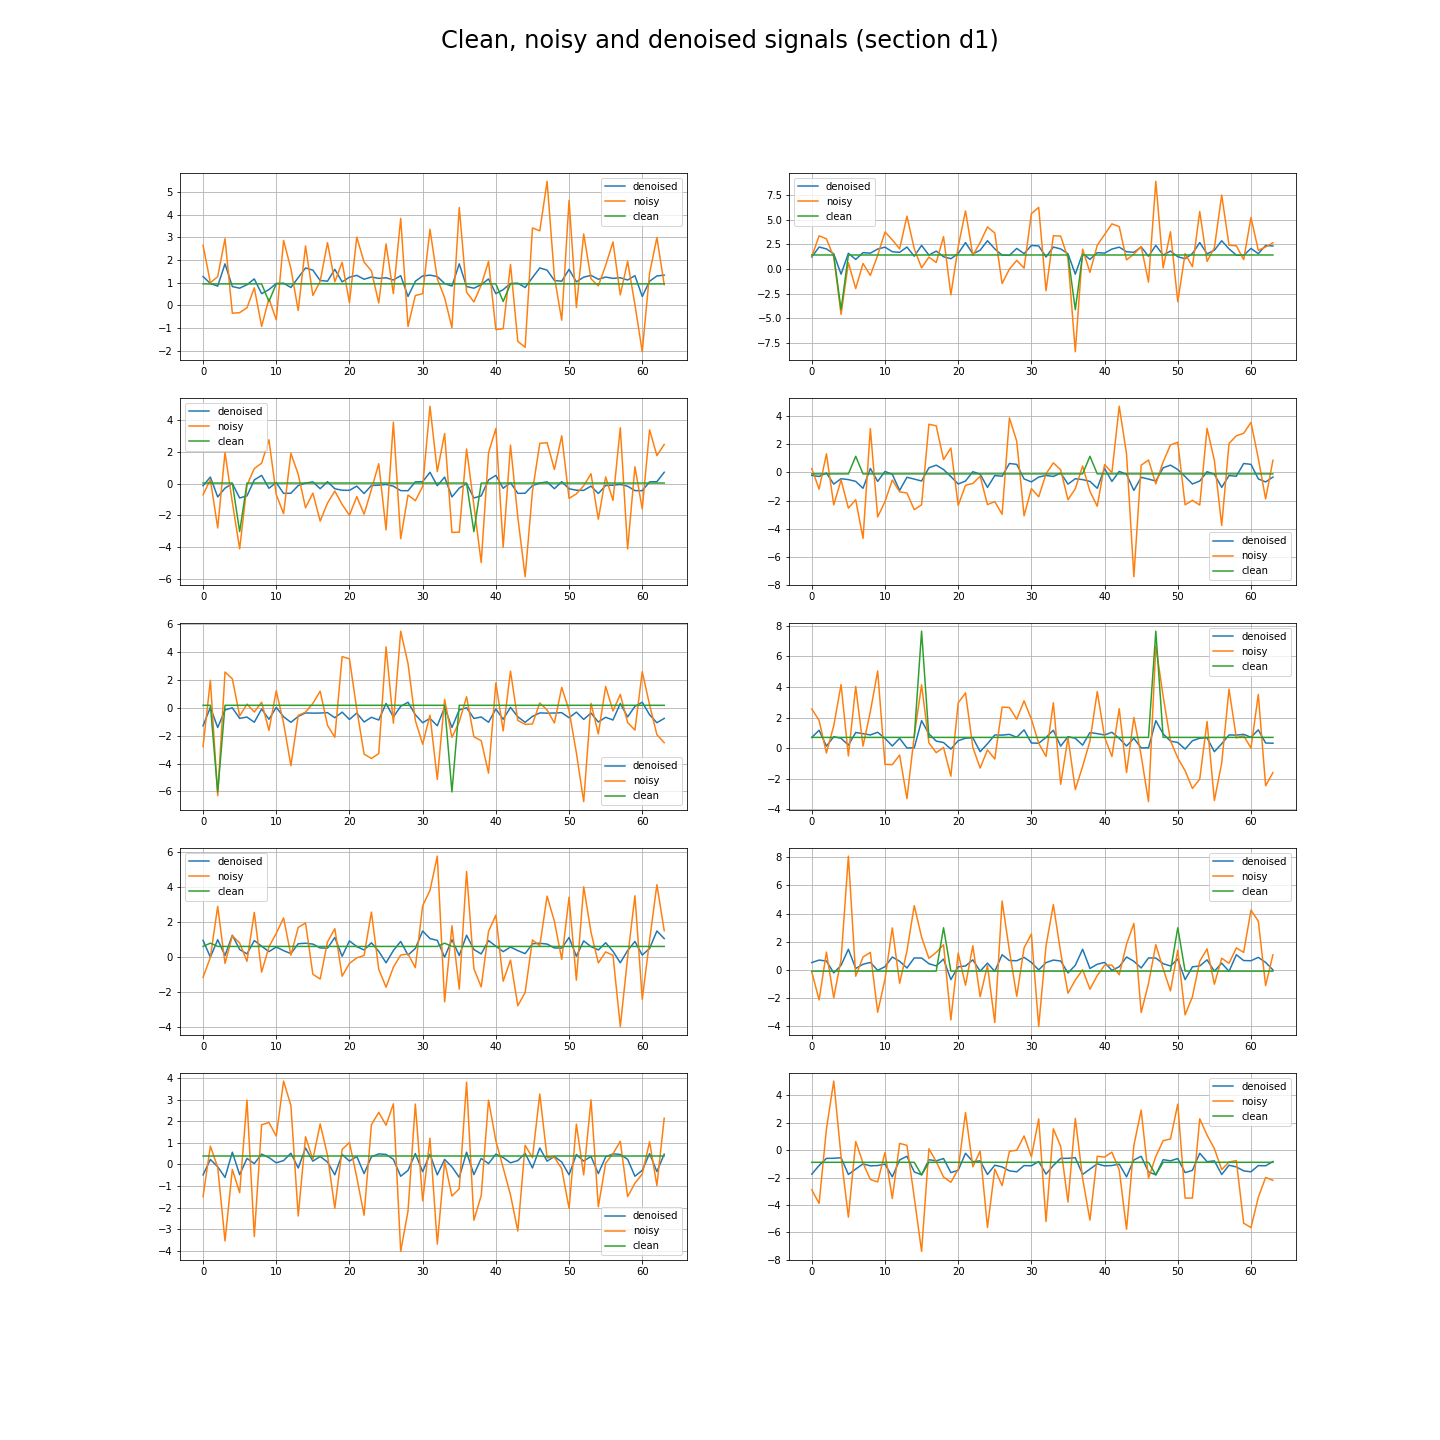
\includegraphics[width=500,keepaspectratio]{samples_d_1.png}
\end{figure}

The mean MSE of all Weiner-denoised signals with respect to the original signals is: 0.447

This is higher than the section b MSE, and can be explained by the higher variance.

\newpage

\subsection*{With linear degradation}

The Wiener filter matrix that we obtained:

\begin{figure}[h]
    \centering
    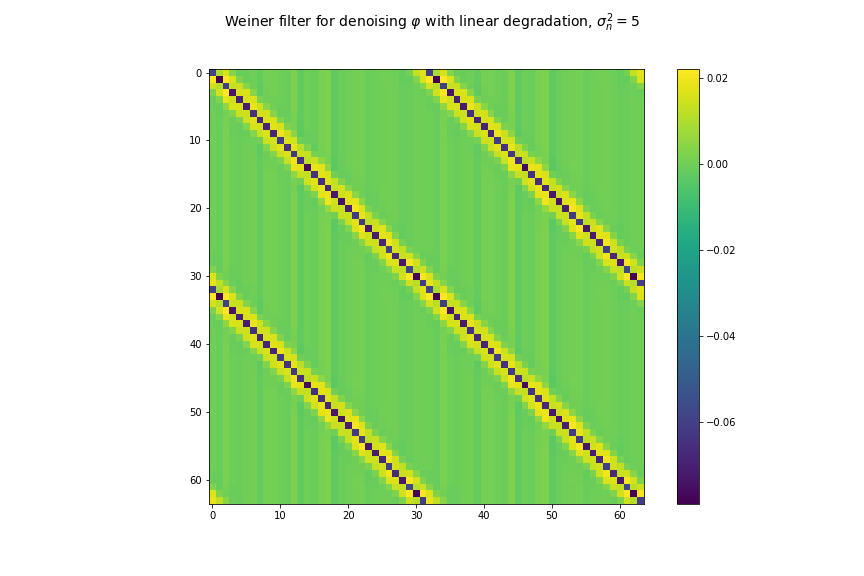
\includegraphics[width=350,keepaspectratio]{p2q1d_weiner_two.png}
\end{figure}

In this section, our linear degradation matrix is a circulant matrix with a first row of \\ \begin{bmatrix}
    -\frac{5}{2} & \frac{4}{3} & -\frac{1}{12} & 0 & \dots & 0 & -\frac{1}{12} & \frac{4}{3}
\end{bmatrix}, so the Weiner filter's formal calculation will be: \\
$W=R_\varphi \cdot H^T \cdot \big(H\cdot R_\varphi \cdot H^T + \sigma_n^2 \cdot I \big) ^ {-1}$

We can also see that the Weiner matrix is circulant, in according to Q4 in the dry part - where if the auto-correlation is circulant, the weiner matrix is circulant.


\newpage 

This is a plot of 10 random signal samples, with their corresponding noisy and denoised signals:

\begin{figure}[h]
    \centering
    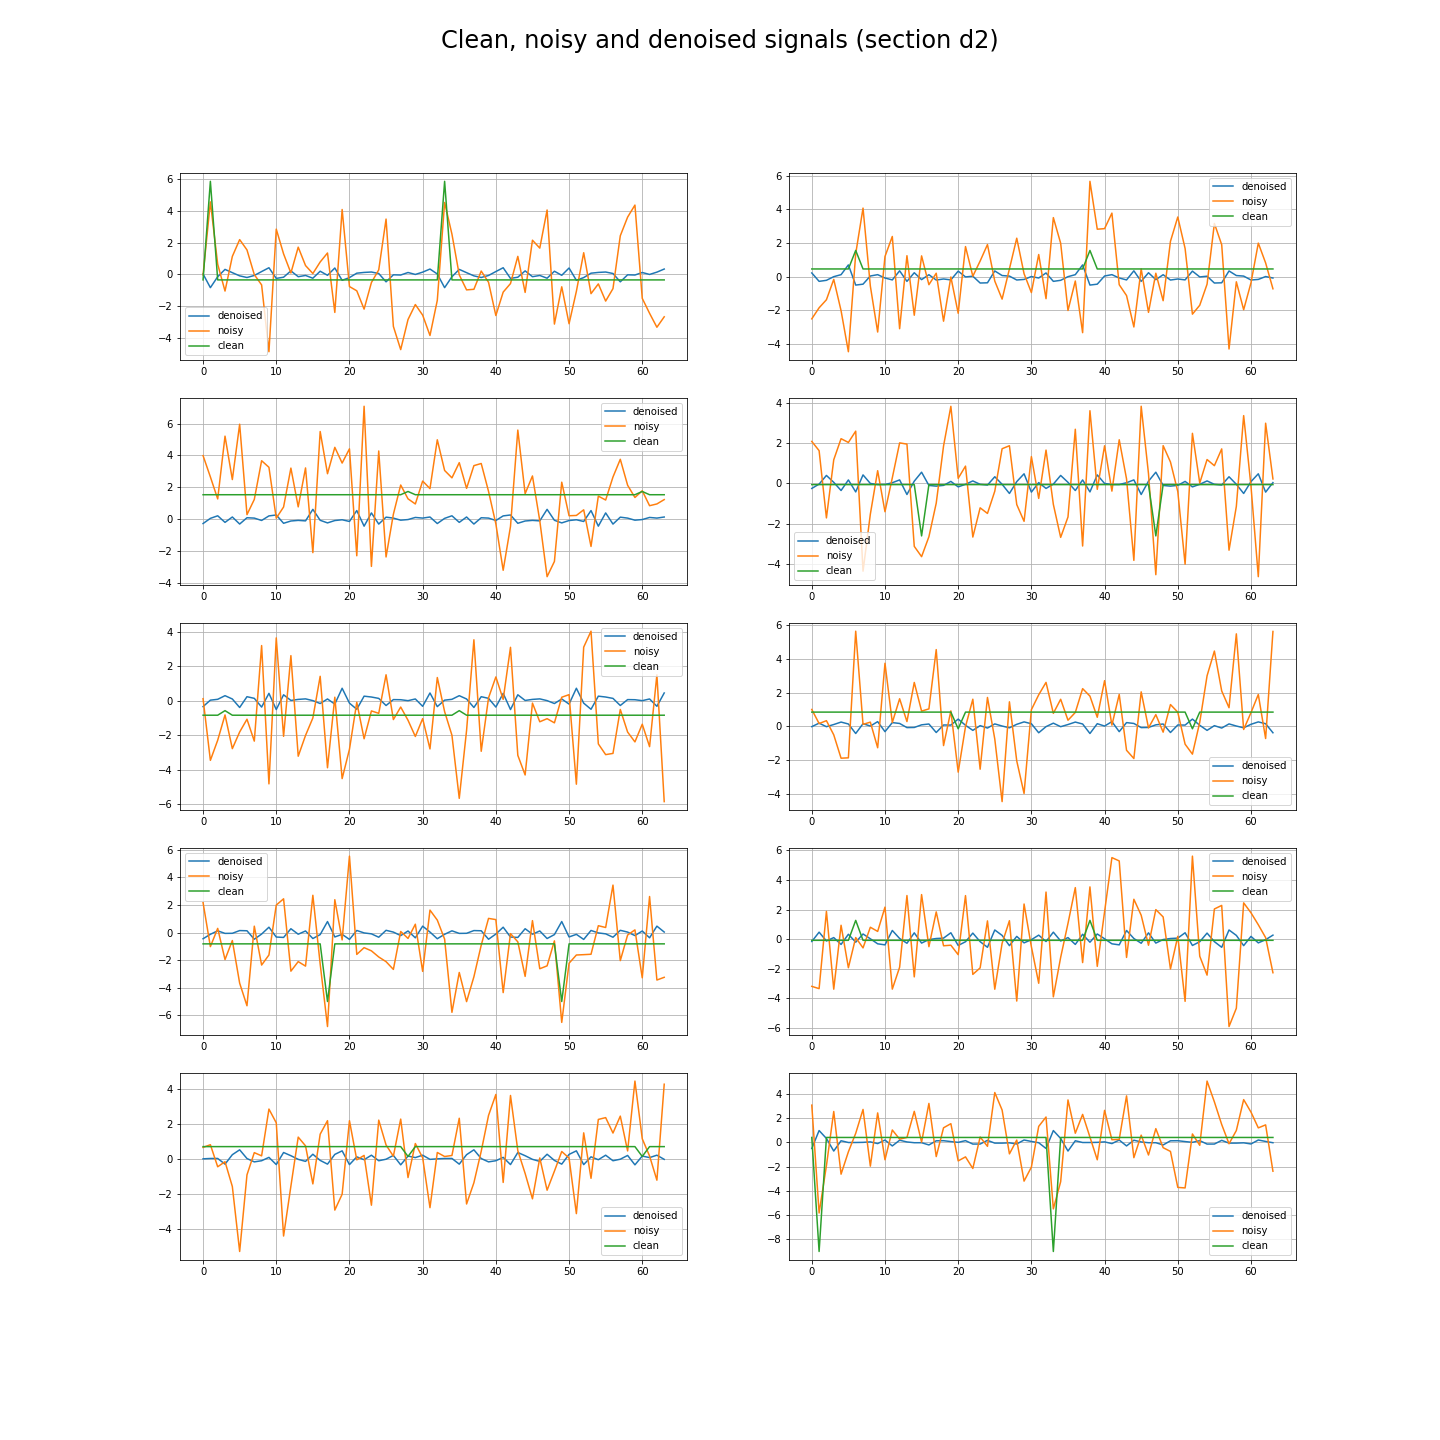
\includegraphics[width=500,keepaspectratio]{samples_d_2.png}
\end{figure}

The mean MSE of all Weiner-denoised signals with respect to the original signals is: 1.173

This is higher than the section c MSE, and can be explained by the higher variance.


\newpage 

\section*{e}

We computed the pseudo-inverse of $H$ with: $np.linalg.pinv$, which is the moore-penrose inverse.

\begin{figure}[h]
    \centering
    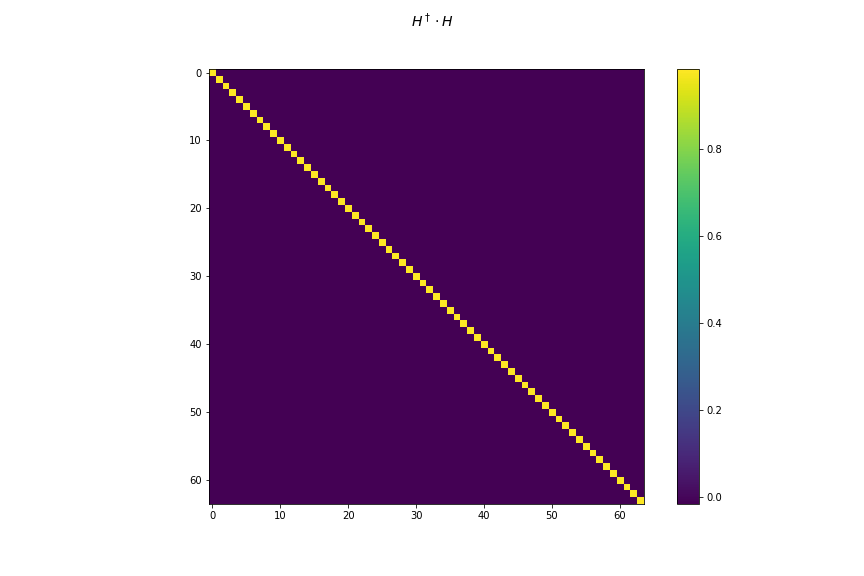
\includegraphics[width=400,keepaspectratio]{hw/hw4/imgs/p2q1e_h_dagger_h.png}
    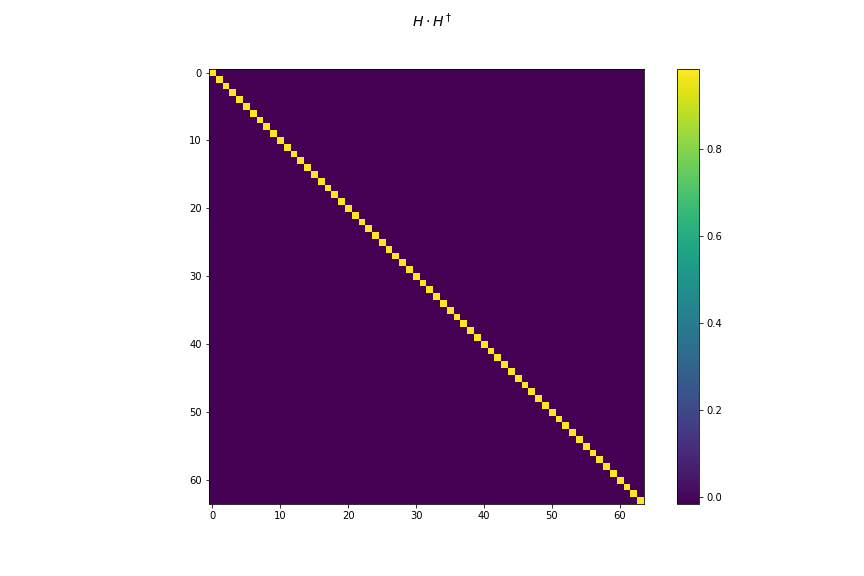
\includegraphics[width=400,keepaspectratio]{hw/hw4/imgs/p2q1e_h_h_dagger.png}
\end{figure}

We can clearly see that $H^\dagger H = HH^\dagger = I$.

\newpage 

For our signals, given the signals:

\begin{align*}
    & \psi_1 = [100, 0, \dots, 0] \\ 
    & \psi_2 = [1, 1, \dots, 1] = ones(N=64) \\
    & \phi_1 = 10\cdot ones(N) + \psi_1 \quad\text{ \# first signal} \\ 
    & \phi_2 = 100\cdot ones(N) + \psi_1 \quad\text{ \# second signal}
\end{align*}

We know from Q1 that the first column if the $DFT^*$ matrix is the eigenvector of $H$ that corresponds to the first eigenvalue - which is 0, and the first column of the $DFT^*$ is $ones(N)$

Therefore, we get that $\lambda=0$ is an eigenvalue of $H^\dagger$ with the eigenvector $ones(N)$ because $H^\dagger$ is circulant and diagonalizable by $DFT^*$.

Because of that, we get that $10\cdot ones(N)$ and $100\cdot ones(N)$ are eigenvectors of $H^\dagger$ with eigenvalue 0. 

So:
\begin{align*}
    & H^\dagger \cdot \phi_1 = H^\dagger \cdot (10ones(N) + \psi_1) = \underbrace{H^\dagger \cdot 10\cdot ones(N)}_{=0} + H^\dagger \cdot \psi_1 = H^\dagger \cdot \psi_1 \\
    & H^\dagger \cdot \phi_2 = H^\dagger \cdot (100ones(N) + \psi_1) = \underbrace{H^\dagger \cdot 100\cdot ones(N)}_{=0} + H^\dagger \cdot \psi_1 = H^\dagger \cdot \psi_1 \\
    & \implies H^\dagger \cdot \phi_1 = H^\dagger \cdot \phi_2 \\
    & Also: \quad \| \phi_1 - \phi_2 \|_2 = 90^2 \cdot 64 \geq 256
\end{align*}

We can compute the norm $\| \phi_1 - \phi_2 \|_2=720$

And the $L2$ norm of $\| H^\dagger \phi_1 - H^\dagger \phi_2 \|_2 = 9.9788\cdot 10^{-9}$, as expected.

\newpage 

The plots we got for the signals:

\begin{figure}[h]
    \centering
    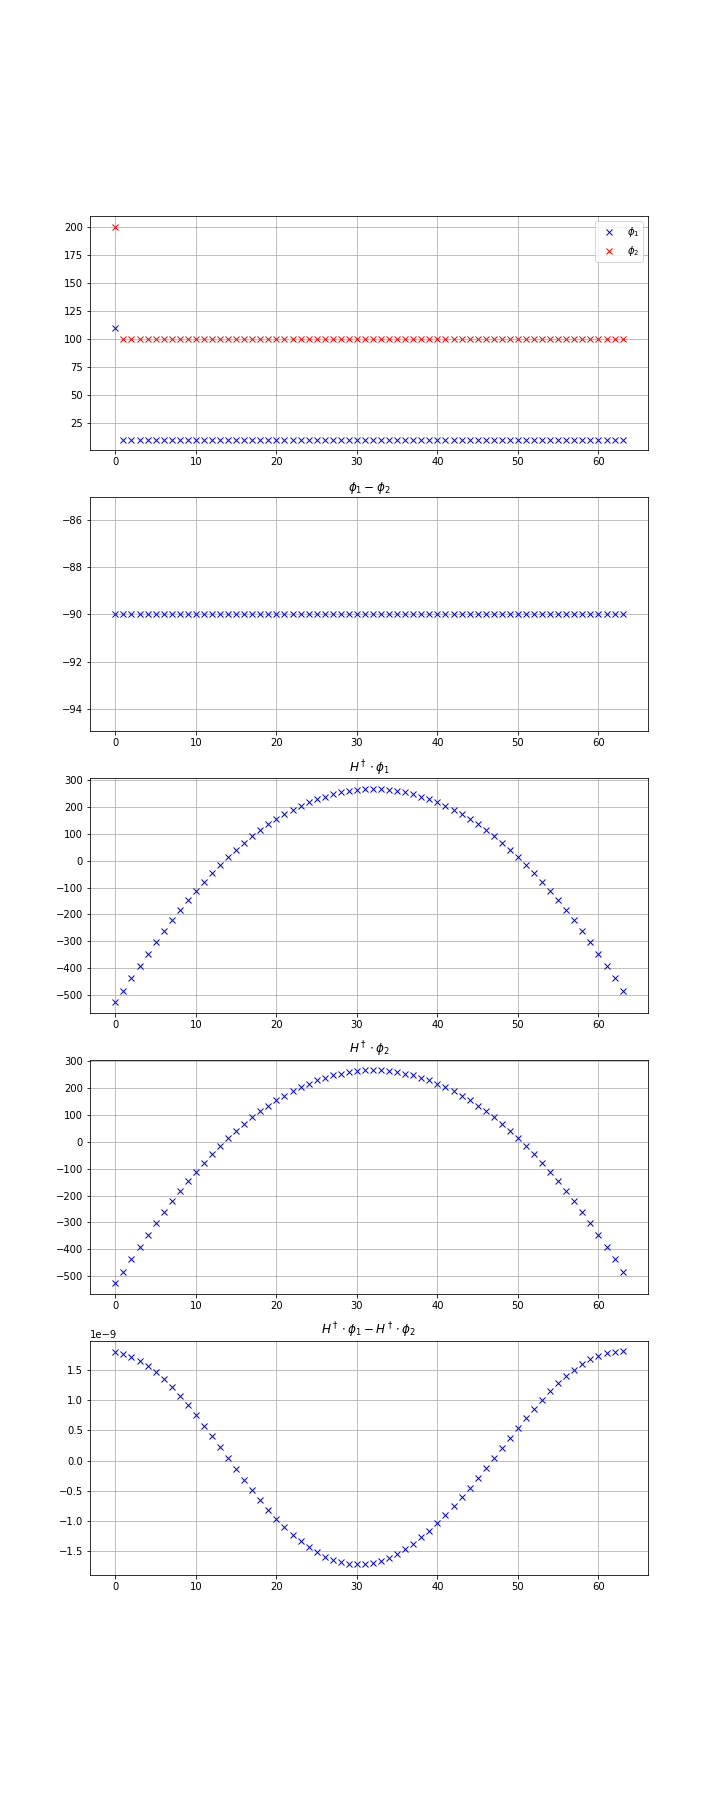
\includegraphics[width=200,keepaspectratio]{p2q1e_signals}
\end{figure}


\end{document}
